% Chapter 2

\chapter{Radares Passivos} % Main chapter title

\label{chap:Chapter2} % For referencing the chapter elsewhere, use \ref{chap:Chapter2} 

%----------------------------------------------------------------------------------------

\section{Contextualização}
Os radares convencionais apresentam uma configuração onde são constituídos por um transmissor e um recetor, normalmente no mesmo local. Neste tipo de radares, um pulso é transmitido em forma de energia eletromagnética, e através do conhecimento do tempo levado pelo pulso a ser transmitido e recebido depois de refletido no alvo e da velocidade de propagação da luz, consegue-se determinar um valor de distância.\par 
Num radar passivo, não existe transmissão de energia eletromagnética durante o seu funcionamento. Ao invés, utiliza iluminadores de oportunidade e compara o seu sinal direto com pequenas alterações que ocorrem no campo eletromagnético por alvos em movimento de forma a detetar um alvo \parencite{Griffiths2017}.\par 
Este sistema radar pode utilizar uma grande variedade de iluminadores, desde sistemas de navegação por satélite (\textit{\gls{GNSS}}) como o \gls{GPS} ou o GLONASS, \textit{routers} de WiFi ou qualquer sistema de transmissão de frequências rádio como \textit{\gls{DVB}} ou estações de rádio. Dito isto, por forma a dimensionar o sistema para o efeito desejado, torna-se necessário uma boa compreensão das mais diversas caraterísticas dos iluminadores, como é falado mais à frente neste capítulo.\par 
Para a finalidade de deteção de alvos a grandes distâncias, os sinais mais eficazes e consequentemente mais utilizados são os que apresentam elevada potência, como transmissores de \gls{VHF} e de televisão digital em \gls{UHF}, não obstante poder-se também utilizar em certos casos outros iluminadores.\par
O cenário típico de um esquema de deteção usando um radar passivo é, como mostrado na Figura \ref{fig:esquema_pcl}, constituído por duas antenas recetoras, uma antena que recebe o sinal direto do iluminador ($S_{ref}$) e outra antena que recebe o sinal que é refletido no alvo ($S_{r}$). O sinal refletido no alvo fornece duas informações importantes para a sua deteção: o \textit{bistatic range}, ou seja, a distância ao alvo, conseguida através da diferença de tempo entre o sinal direto e o sinal refletido; e o \textit{Doppler}, que é o desvio de frequência que um alvo em movimento cria no sinal que é refletido devido à sua velocidade. Estes conceitos são discutidos mais à frente neste capitulo. \par

\begin{figure}[h]
\centering
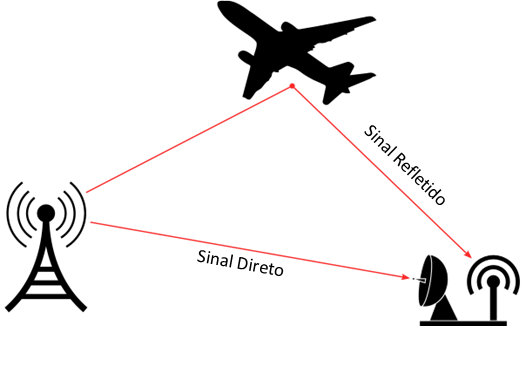
\includegraphics[scale=0.7]{chapters/ch2/assets/esquema_pcl}
\caption[Esquema Geometria Radar Passivo]{Esquema da geometria de um radar passivo}
\label{fig:esquema_pcl}
\end{figure}

O conceito do radar passivo é fazer uma relação cruzada, ou, como mais conhecido o termo, \textit{cross-correlation} entre o sinal direto e o sinal refletido em função das variáveis \textit{delay-time} que pode ser transformado em \textit{bistatic range} e o desvio de \textit{Doppler}. A \textit{cross-correlation}, de forma simples, é uma medida de similaridade entre dois sinais aplicando um atraso num deles, que neste caso, para além do atraso (\textit{delay-time}), também é feita para os diferentes \textit{Doppler}, ou seja, em duas dimensões. No entanto, na prática existem processos analíticos mais eficientes, visto que fazer a \textit{cross-correlation} a duas dimensões em tempo real torna o processo muito pesado computacionalmente.



\subsection{Geometrias Radar}
Podemos classificar os radares quanto à localização dos transmissores e recetores. O ângulo $\beta$ que estes formam, sendo o seu centro o alvo, determina o tipo de geometria \parencite{Baker2019}. Se $\beta <20^{\circ}$, o transmissor e o recetor encontram-se perto ou no mesmo sítio, então estamos perante uma geometria monostática (Figura \ref{fig:monostatic}). Quando o transmissor e recetor estão mais afastados e formam um ângulo com centro no recetor dentro dos seguintes limites, $20^{\circ}<\beta <145^{\circ}$, a geometria é bistática (Figura \ref{fig:bistatic}). Para situações particulares, em que o alvo se encontra a uma cota baixa em relação à linha imaginária que une o transmissor e o recetor ($145^{\circ}<\beta <180^{\circ}$), estamos perante uma geometria \textit{Forward Scatter} (Figura \ref{fig:fsc}).\par   

\begin{figure}[h]
\centering
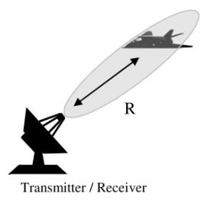
\includegraphics[scale=0.8]{chapters/ch2/assets/monostatic}
\caption[Geometria Monostática]{Geometria Monostática}
\label{fig:monostatic}
\end{figure}

\begin{figure}[h]
\centering
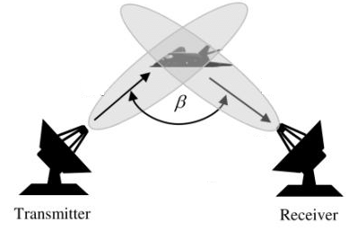
\includegraphics[scale=0.8]{chapters/ch2/assets/bistatic}
\caption[Geometria Bistática]{Geometria Bistática}
\label{fig:bistatic}
\end{figure}

\begin{figure}[h]
\centering
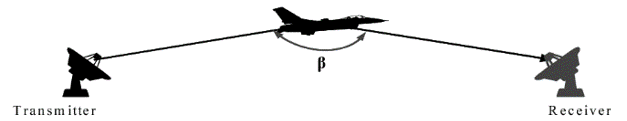
\includegraphics[scale=0.7]{chapters/ch2/assets/fsc}
\caption[Geometria \textit{Forward Scatter}]{Geometria \textit{Forward Scatter}}
\label{fig:fsc}
\end{figure}

Os radares passivos, como já discutido, têm a vantagem de não transmitirem um sinal, e ao invés usar um sinal a ser transmitido por outra fonte. Isto implica que o transmissor e o recetor não estejam no mesmo sítio nem perto, logo, quando se fala em radares passivos, assume-se uma geometria bistática.



\subsection{Alcance Bistático e \textit{Doppler}}
Como falado no ínicio deste capítulo, o alcance bistático, ou \textit{bistatic range} e o desvio de \textit{Doppler} são varáveis fundamentais para qualquer sistema radar e isso não exclui o radar passivo.

\subsection{Formação de Imagem}

